\section{Pipeline}

\tikzstyle{process} = [rectangle, rounded corners, minimum width=2cm, minimum height=1cm,text centered, draw=black, fill=gray!50]
\tikzstyle{decision} = [diamond, minimum width=3cm, minimum height=1cm, text centered, draw=black, fill=green!30]

\begin{figure}[ht]
    \centering
    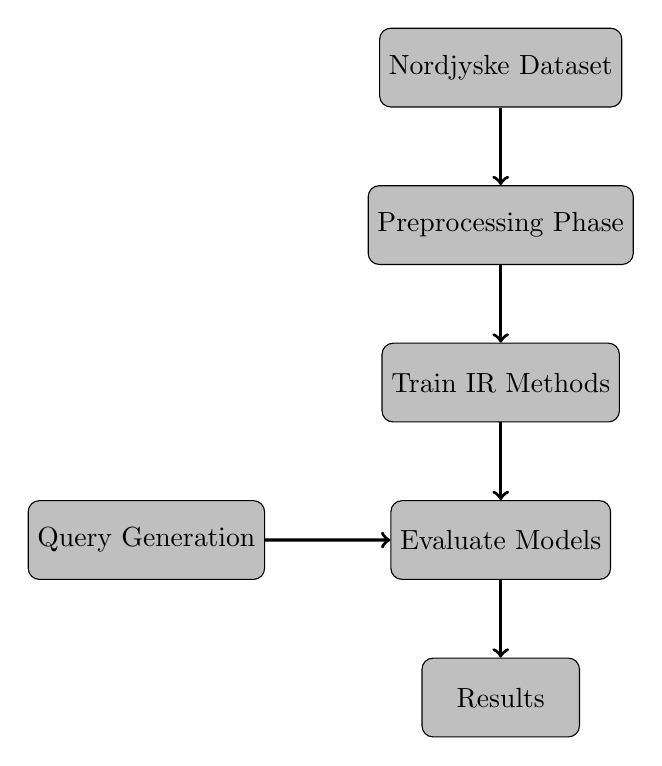
\begin{tikzpicture}[node distance=2cm]
    %\draw[step=1cm,gray,very thin] (-8,-8) grid (8,8);
	\node (Dataset) [process] {Nordjyske Dataset};
	\node (Cleaning)[process, below of=Dataset] {Preprocessing Phase};
	\node (Training) [process, below of=Cleaning] {Train IR Methods};
	\node (Cluster PR) [process, below of=Training] {Evaluate Models};
	\node (Query) at (-4.5, -6) [process] {Query Generation};
	\node (Result) [process, below of=Cluster PR] {Results};
	\draw [->, very thick] (Dataset) edge (Cleaning); 
	\draw [->, very thick] (Cleaning) edge (Training);
	\draw [->, very thick] (Training) edge (Cluster PR);
	\draw [->, very thick] (Cluster PR) edge (Result);
	\draw [->, very thick] (Query) edge (Cluster PR);
\end{tikzpicture}
	\caption{The method visualized as a flowchart, where a dataset consisting of articles is processed into a list of ranked results.}
    \label{fig:process_figure}
\end{figure}

The pipeline of our framework is divided into five different phases which are displayed in \autoref{fig:pipeline}.

\subsection{Article dataset}
We have an dataset consisting of articles from the media group Nordjyske, whose primary focus is maintaining a variety of local newspapers within the North Jutland region of Denmark. 
The data is from 2017-2019, where a total of ~270.000 articles have been extracted from their database.

\subsection{Preprocessing}
The articles are on the format:
\begin{itemize}
	\item Id
	\item Headline
	\item Body
\end{itemize}
When training the LDA model, we concatenate the Headline and Body for simplicity.
The preprocessing phase is described further in detail in \todo[inline]{ref til preprocessing}.
This phase applies some processes to simplify the dataset and remove redundant noise from the data. 
After the preprocessing phase, we are left with 130.000 articles.
